\documentclass[12pt]{article}
% \pagestyle{empty}
\usepackage{graphicx}
\usepackage{amsmath}
\usepackage{amsfonts}
\usepackage{listings}
\usepackage{color}
\usepackage{textcomp}
\definecolor{listinggray}{gray}{0.9}
\definecolor{lbcolor}{rgb}{0.9,0.9,0.9}
\lstset{
	backgroundcolor=\color{lbcolor},
	tabsize=4,
	rulecolor=,
	language=Python,
        basicstyle=\scriptsize,
        upquote=true,
        aboveskip={1.5\baselineskip},
        columns=fixed,
        showstringspaces=false,
        extendedchars=true,
        breaklines=true,
        prebreak = \raisebox{0ex}[0ex][0ex]{\ensuremath{\hookleftarrow}},
        frame=single,
        showtabs=false,
        showspaces=false,
        showstringspaces=false,
        identifierstyle=\ttfamily,
        keywordstyle=\color[rgb]{0,0,1},
        commentstyle=\color[rgb]{0.133,0.545,0.133},
        stringstyle=\color[rgb]{0.627,0.126,0.941},
}

\title{Nonlinear FEM Homework 5}
\author{Truman Ellis}
\date{}

\begin{document}
\maketitle

The natural frequencies of the system can be computed by solving for the
square root of the eigenvalues of $M^{-1}K=K$. A simple calculation yields the
following eigenvalues,
\[
\lambda_1 = \frac{10002-\sqrt{10002^2-40000}}{2}\approx0.999900
\]
\[
\lambda_2 = \frac{10002+\sqrt{10002^2-40000}}{2}\approx10001.0\,,
\]
from which we can calculate
\[
\omega_1 \approx 0.99995
\]
\[
\omega_2 \approx 100.005\,.
\]
Therefore $t_1=\frac{2\pi}{\omega_1}\approx 2\pi$.

Then we get the following solutions for Central Difference, Trapezoid rule,
and Damped Newmark, respectively for Exercise 16. 

For Exercise 17 we get $\omega_1=0.707098$, and $\omega_2=141.423$, and
similar results follow below.

In both problems it appears that Central Differences are unstable, the
Trapezoid rule keeps the spurious modes, but doesn't allow them to grow, and
Damped Newmark kills the spurious modes.

\begin{figure}[h!]
\centering
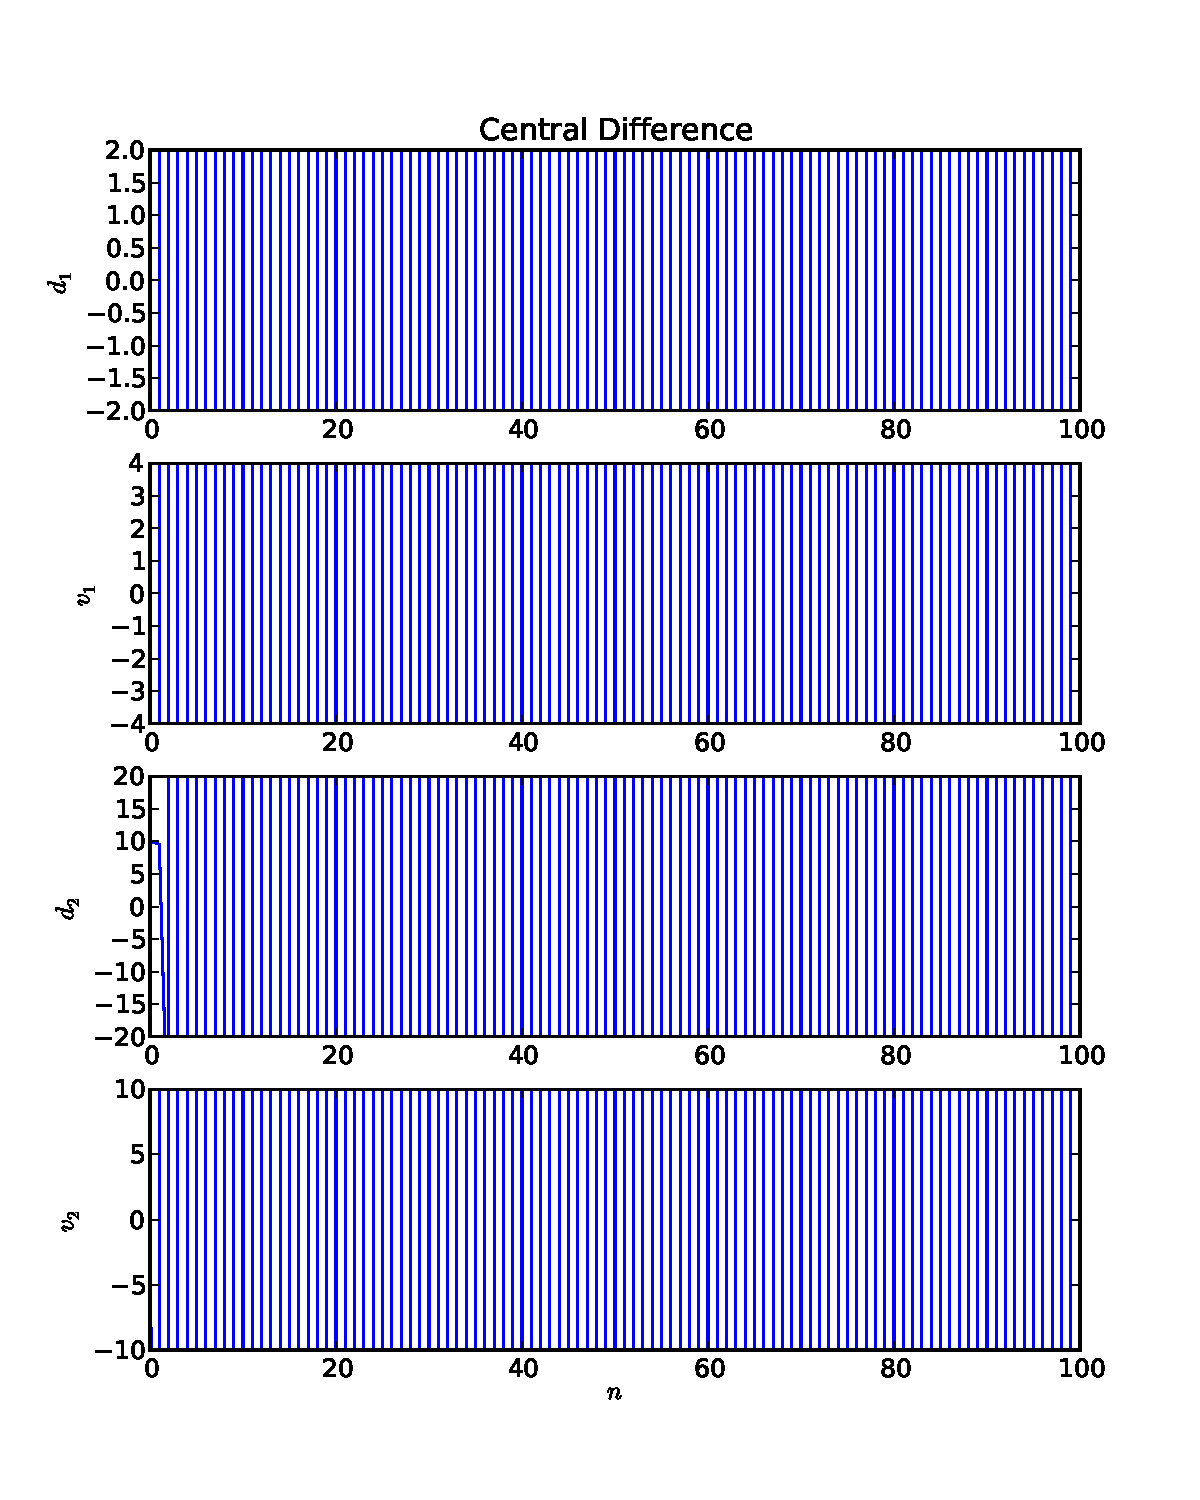
\includegraphics[height=0.9\textheight]{cd1.pdf}
\caption{Exercise 16, Central Difference}
\end{figure}

\begin{figure}[h!]
\centering
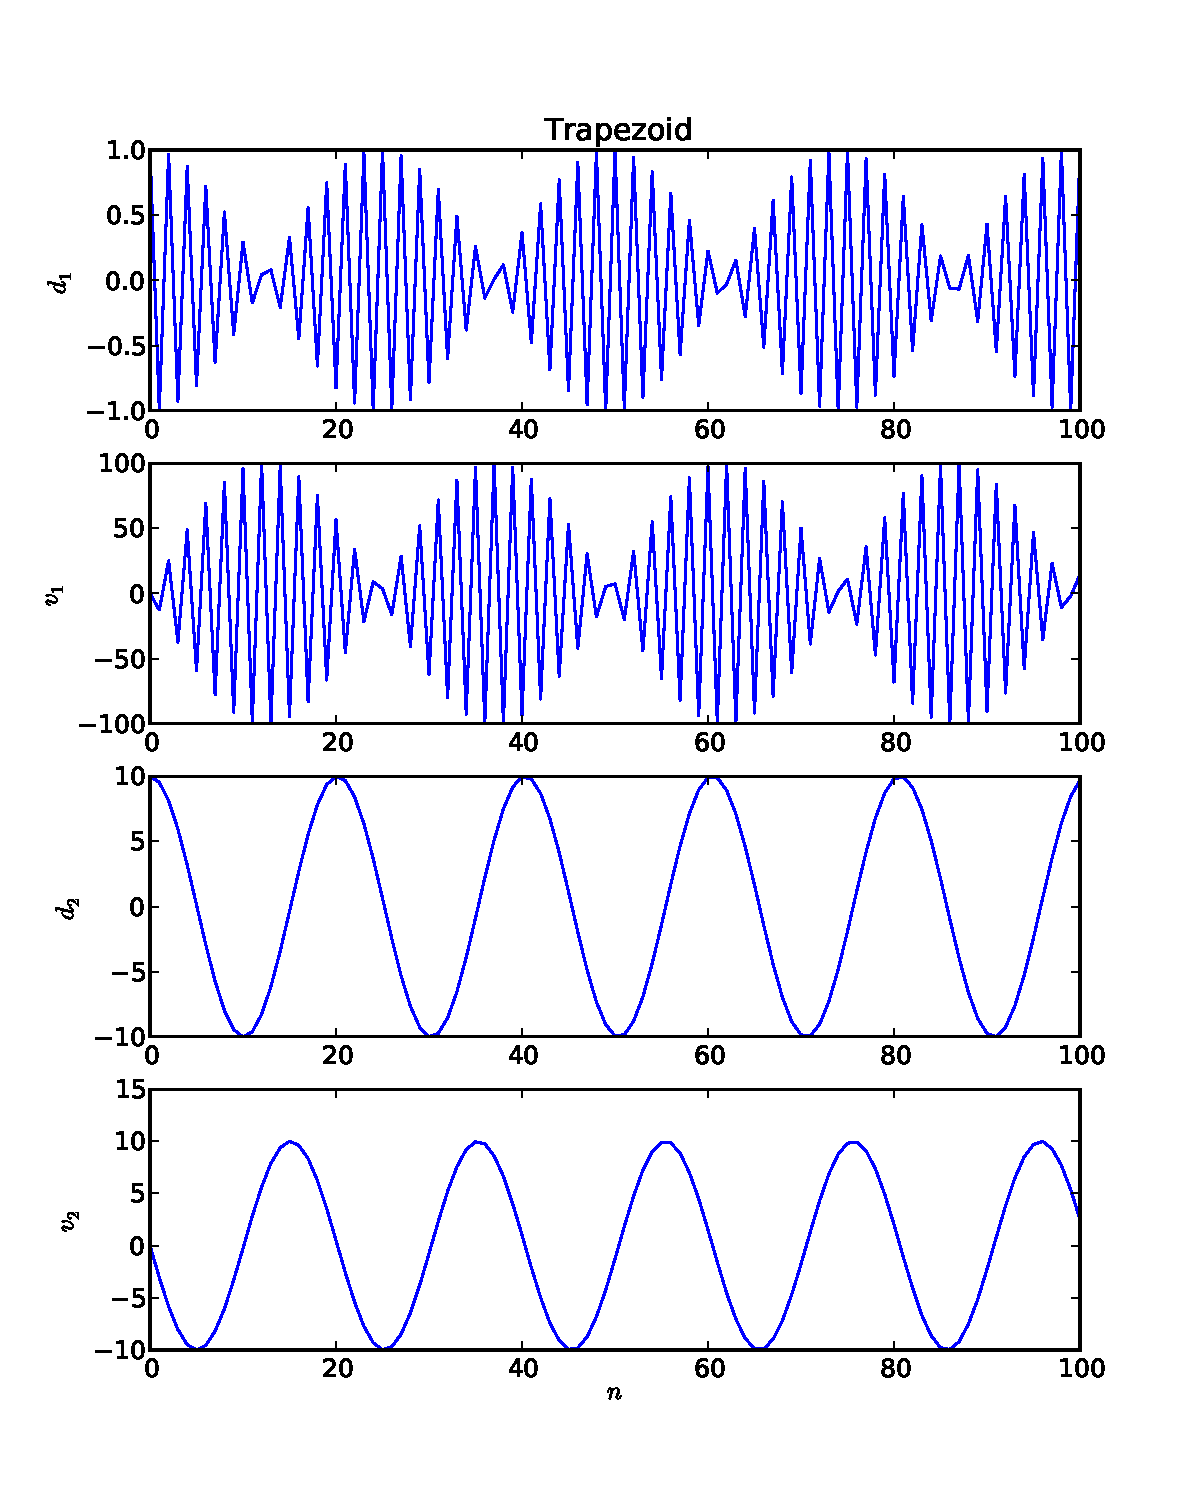
\includegraphics[height=0.9\textheight]{t1.pdf}
\caption{Exercise 16, Trapezoid Rule}
\end{figure}

\begin{figure}[h!]
\centering
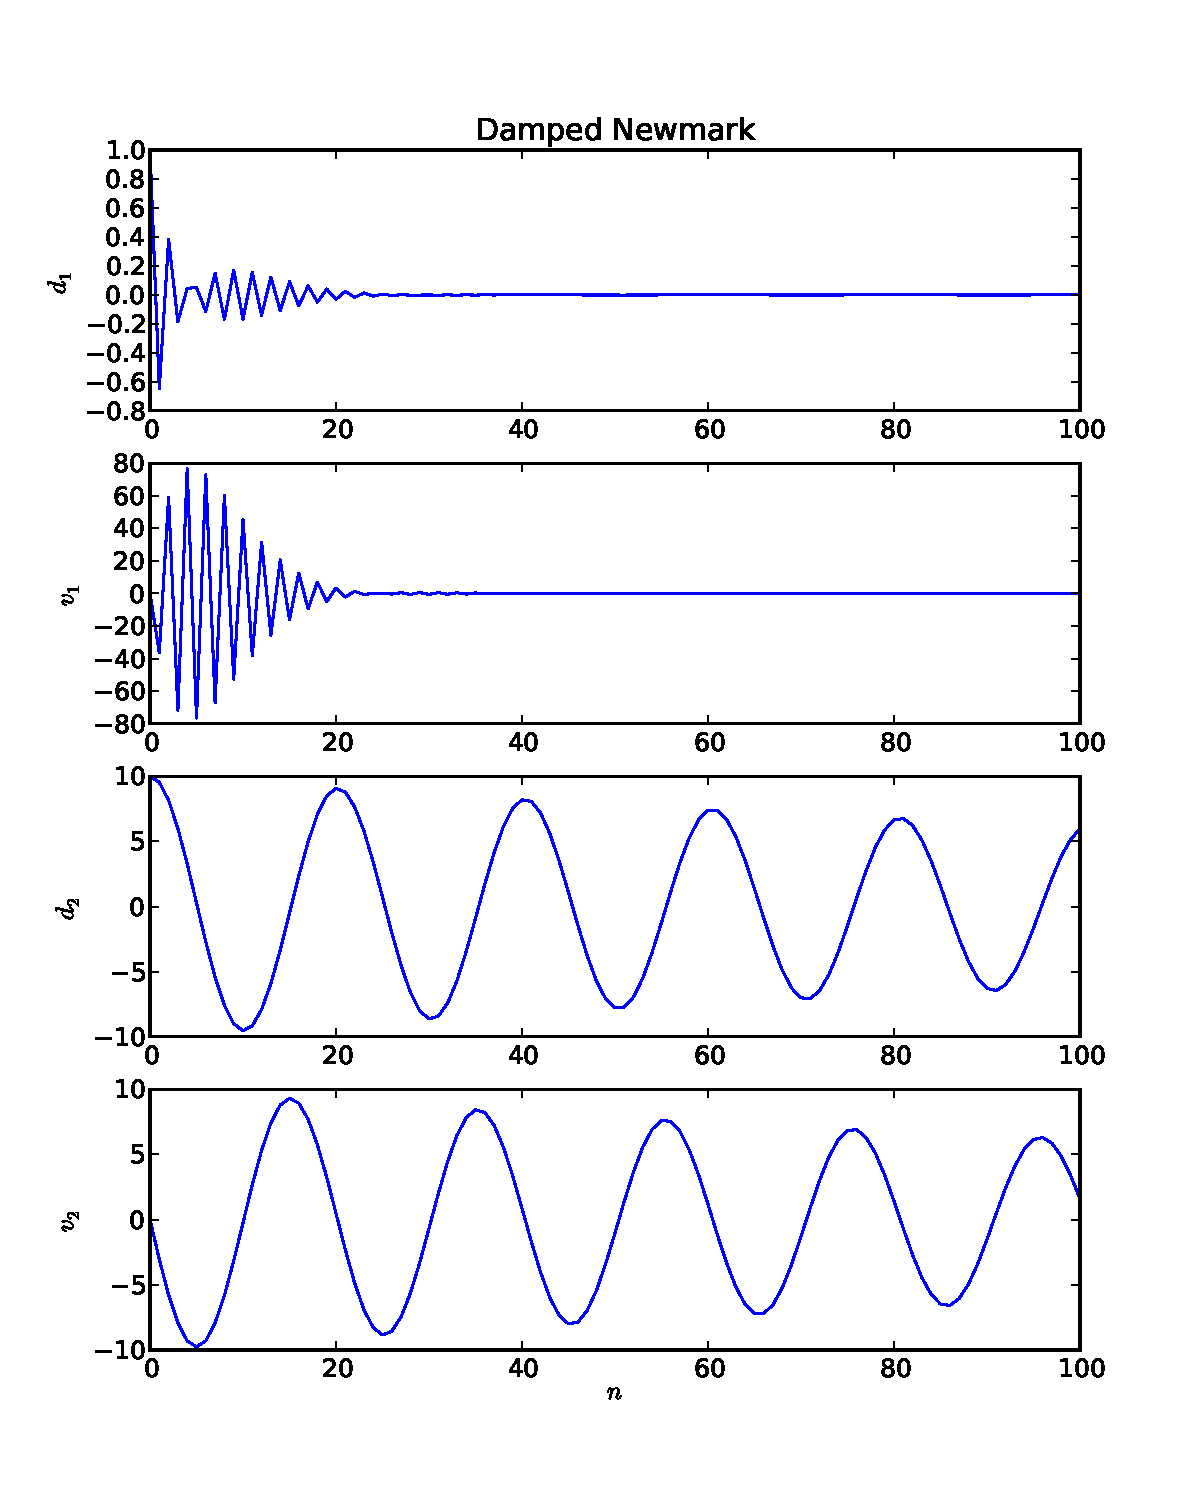
\includegraphics[height=0.9\textheight]{dn1.pdf}
\caption{Exercise 16, Damped Newmark}
\end{figure}

\begin{figure}[h!]
\centering
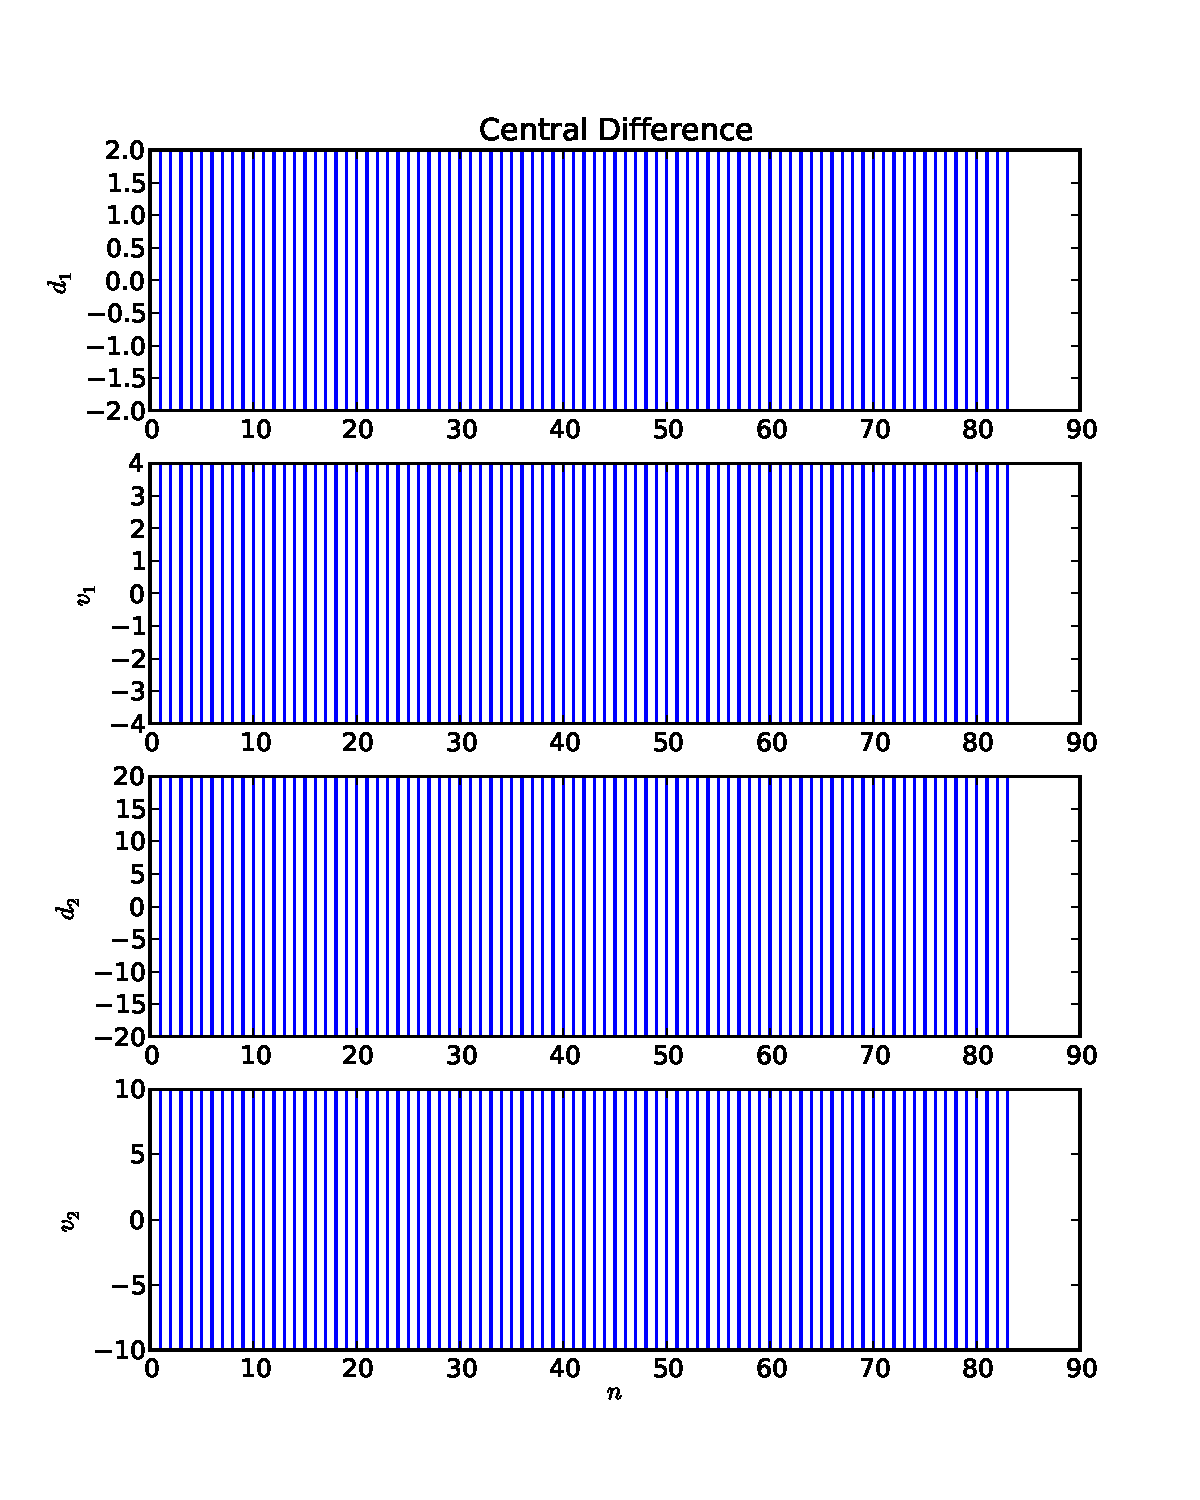
\includegraphics[height=0.9\textheight]{cd2.pdf}
\caption{Exercise 17, Central Difference}
\end{figure}

\begin{figure}[h!]
\centering
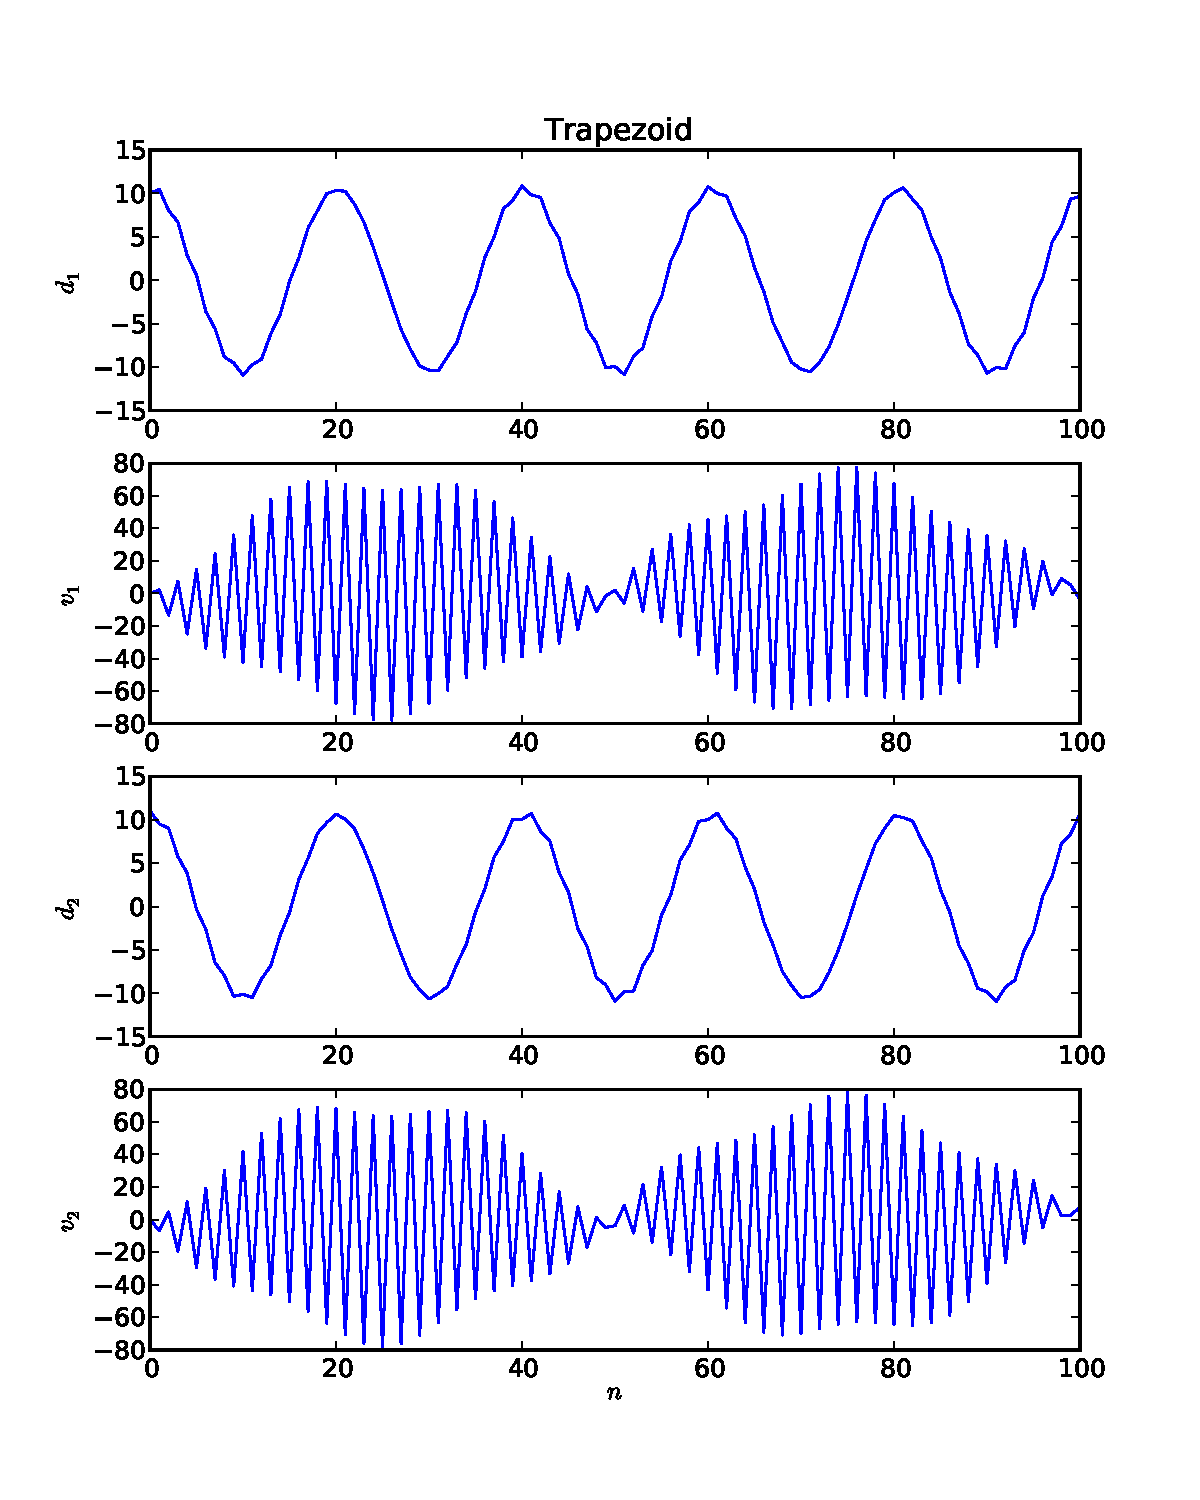
\includegraphics[height=0.9\textheight]{t2.pdf}
\caption{Exercise 17, Trapezoid Rule}
\end{figure}

\begin{figure}[h!]
\centering
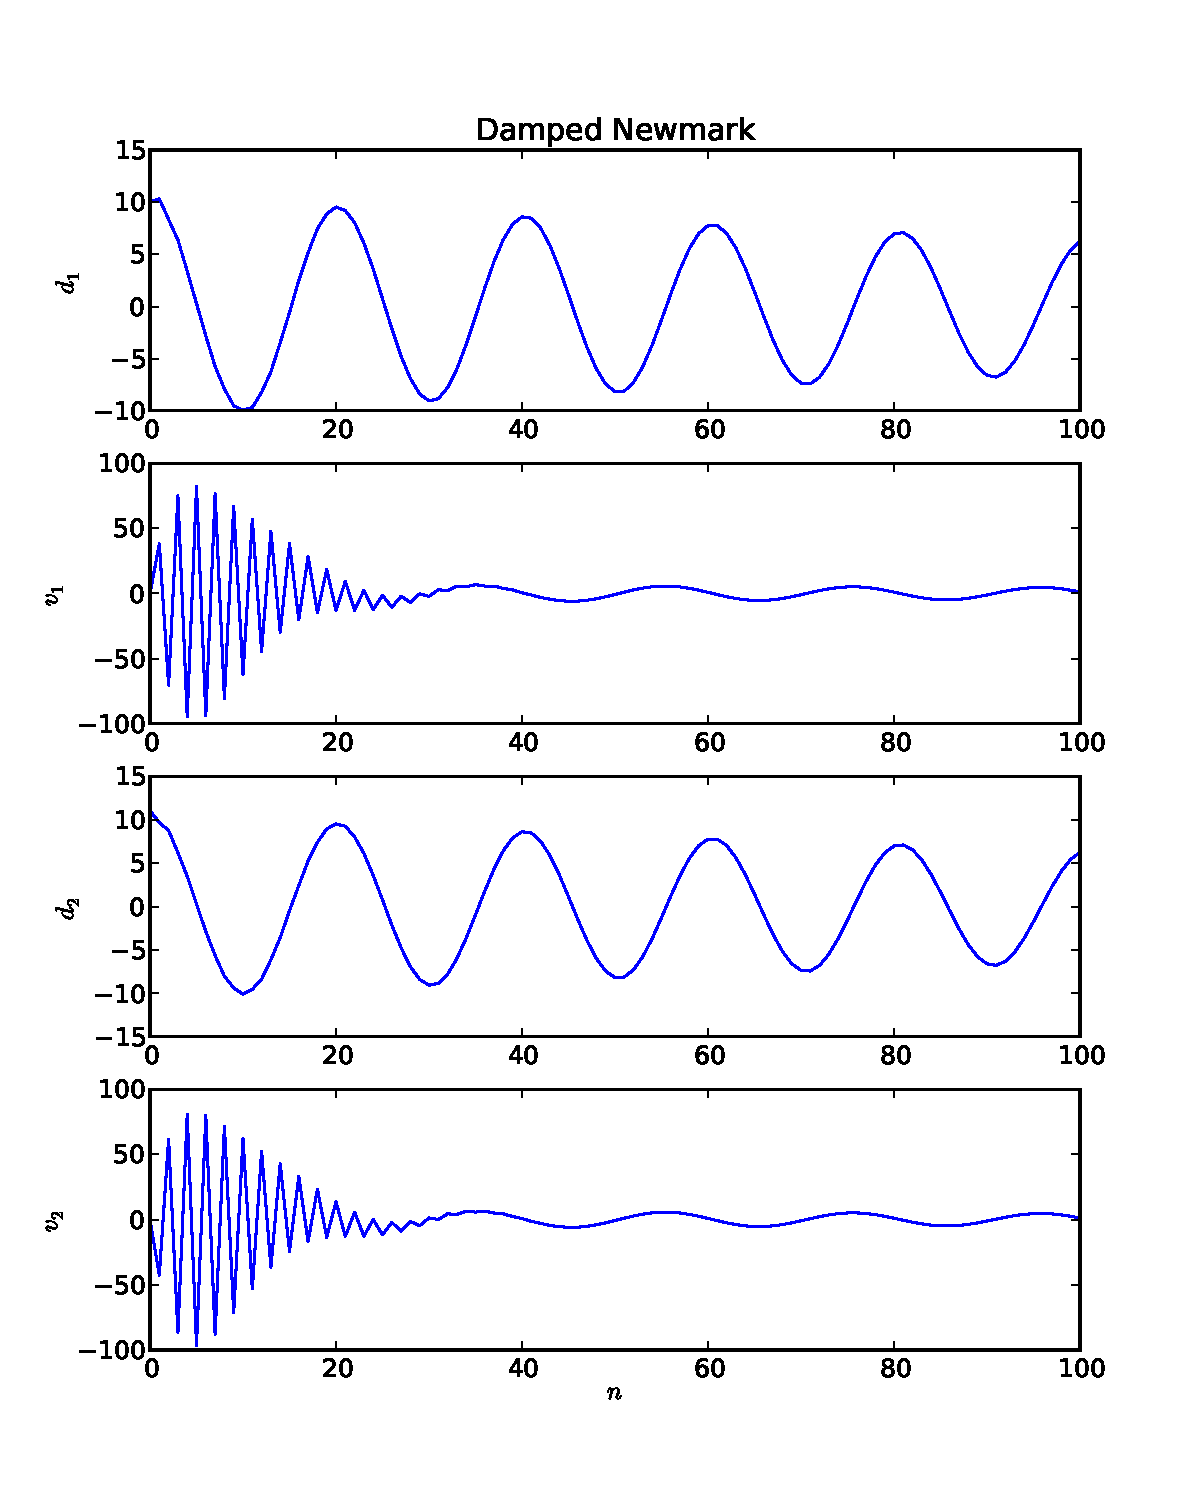
\includegraphics[height=0.9\textheight]{dn2.pdf}
\caption{Exercise 17, Damped Newmark}
\end{figure}

\clearpage
\newpage
\lstinputlisting[language=Python,title={HW10.py}]{HW10.py}

\end{document}
